\documentclass[tikz, border=1mm]{standalone}
\begin{document}
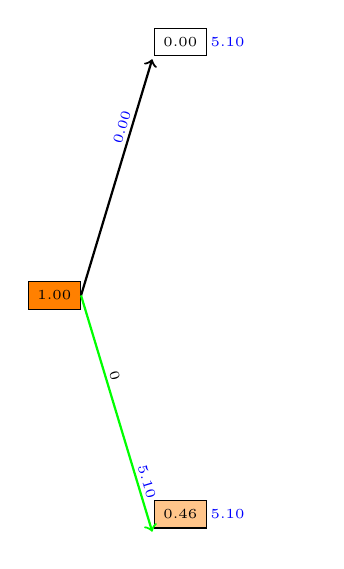
\begin{tikzpicture}
\tikzstyle{between} = [rectangle, minimum height=0.10cm, minimum width=0.70cm, draw opacity=0]
\tikzstyle{qval}    = [rectangle, text centered, text width=2cm]
\node[between] at (-8.40, 3.00) (1_b_0){};
\node[between] at (-8.40, -3.00) (1_b_1){};
\node[rectangle, text centered, draw=black, minimum height=0.20cm, minimum width=0.45cm, fill=orange, fill opacity=1.00, draw opacity=1, text opacity=1] at (-10.00, 0.00) (0_s_0) {\tiny 1.00};
\node[rectangle, text centered, draw=black, minimum height=0.20cm, minimum width=0.45cm, fill=orange, fill opacity=0.00, draw opacity=1, text opacity=1] at (-8.40, 3.22) (1_s_0) {\tiny 0.00};
\node[qval] at (-7.80, 3.22) () {\tiny \textcolor{blue}{5.10}};
\node[rectangle, text centered, draw=black, minimum height=0.20cm, minimum width=0.45cm, fill=orange, fill opacity=0.46, draw opacity=1, text opacity=1] at (-8.40, -2.78) (1_s_2) {\tiny 0.46};
\node[qval] at (-7.80, -2.78) () {\tiny \textcolor{blue}{5.10}};
\draw[->, thick, black] (0_s_0.east) -- (1_b_0.west) node [pos=0.70, above=-0.2em, sloped, font=\tiny] () {\textcolor{blue}{0.00}};
\draw[->, thick, green] (0_s_0.east) -- (1_b_1.west) node [pos=0.35, above=-0.2em, sloped, font=\tiny] () {\textcolor{black}{0}} node [pos=0.80, above=-0.2em, sloped, font=\tiny] () {\textcolor{blue}{5.10}};
\end{tikzpicture}
\end{document}